\documentclass[11pt,a4paper]{article}
%\documentclass[11pt,a4paper,twoside]{article}
\usepackage[utf8]{inputenc}
\usepackage[french]{babel}
\usepackage[T1]{fontenc}

\usepackage{amsmath}
\usepackage{amsfonts}
\usepackage{amssymb}

\newcommand{\TitreMatiere}{Architecture des Ordinateurs}
\newcommand{\TitreSeance}{Conversions des Flottants}
\newcommand{\NumeroTD}{IEEE 754}
\newcommand{\DateCours}{Octobre 2023}
\newcommand{\AnneeScolaire}{2023-2024}
\newcommand{\Organisation}{EPITA}
\newcommand{\NomAuteurA}{Fabrice BOISSIER}
\newcommand{\MailAuteurA}{fabrice.boissier@epita.fr}
\newcommand{\NomAuteurB}{ }
\newcommand{\MailAuteurB}{ }
\newcommand{\DocKeywords}{Architecture}
\newcommand{\DocLangue}{fr} % "en", "fr", ...

\usepackage{MetalCourseBooklet}

% Babel ne traduit pas toujours bien les tableaux et autres
\renewcommand*\frenchfigurename{%
    {\scshape Figure}%
}
\renewcommand*\frenchtablename{%
    {\scshape Tableau}%
}

% Ne pas afficher le numéro de la légende sur tableaux et figures
\captionsetup{format=sanslabel}


\usepackage{xlop}  % Ajout des jolies divisions posées :   \opdiv{25}{7}  \opidiv{25}{7}
%\usepackage{pstricks}  % style pour xlop

\begin{document}

\EncadreTitre

\bigskip


%\begin{center}
%\begin{tabular}{p{5cm} p{11cm}}
%\textbf{Commandes étudiées :} & \texttt{sh}, \texttt{bash}, \texttt{man}, \texttt{ls}, \texttt{mkdir}, \texttt{touch}, \texttt{chmod}, \texttt{mv}, \texttt{rm}, \texttt{rmdir}, \texttt{cat}, \texttt{file}, \texttt{which}, \texttt{which}\\
%
%\textbf{Builtins étudiées :} & \texttt{pwd}, \texttt{cd}, \texttt{exit}, \texttt{logout}, \texttt{echo}, \texttt{umask}, \texttt{type}, \texttt{>}, \texttt{>{}>}, \texttt{<}, \texttt{<{}<}, \texttt{|}\\
%
%\textbf{Notions étudiées :} & Shell, Manuels, Fichiers, Répertoires, Droits, Redirections\\
%\end{tabular}
%\end{center}

\bigskip


Ce document a pour objectif de vous familiariser avec les conversions entre plusieurs bases pour les flottants en respectant la norme IEEE 754.

\bigskip

La plupart des conversions que nous effectuerons seront entre les bases 2, 10, et 16 pour les flottants IEEE 754.

Pour rappel, un nombre en indice peut indiquer la base ($ 10_{2} $ indique du binaire, $ 10_{10} $ indique du décimal, ...) tout comme un symbole en préfixe ($ \% $ indique du binaire, et $ \$ $ indique de l'hexadécimal).
Sans symbole particulier, on considère qu'il s'agit de la base 10 usuelle.

\bigskip

%%%%%%%%%%%%%%%%%%%%%%%%%%%%%%%%%%%%%%

\section{Représentation des flottants}

\bigskip

Les flottants concernent les nombres à virgules.
Représenter et manipuler des nombres à virgules n'est pas aisé dans le sens où plusieurs questions se posent : combien de nombres après la virgule faut-il gérer ? Quel est le plus petit pas/décalage supporté par un ordinateur ? ...
Ces questions touchent au principal problème rencontré par l'informatique dans le traitement des données scientifiques : la \og précision \fg{} .

\bigskip

La précision décrit combien de bits seront utilisés pour représenter les nombres flottants.
Dans la norme IEEE 754, il existe plusieurs formats pour représenter les flottants, dont la \textit{simple précision} (sur 32 bits), la \textit{double précision} (sur 64 bits), et la \textit{double précision étendue} (sur 80 bits).

\bigskip

Parmi les contraintes que vous aviez déjà vus, un nombre entier codé sur 8 bits ne pourra pas aller au delà de la valeur $ 256 $ : si on a $ \% \, 1111 \; 1111 $ et qu'on lui ajoute $ 1 $, alors de la valeur 256, on repassera à 0.
Ce phénomène s'appelle un \textit{integer overflow} (dépassement d'entier), qu'il ne faut pas confondre avec les autres types d'\textit{overflows} (stack overflow, buffer overflow).
Dans le cas des flottants, ce type de dépassement est également possible, mais, il existe également le cas inverse : l'\textit{underflow} où l'on cherche à représenter une valeur trop petite pour la précision choisie.

\medskip

\begin{center}
\begin{figure}[ht!]
\centering{
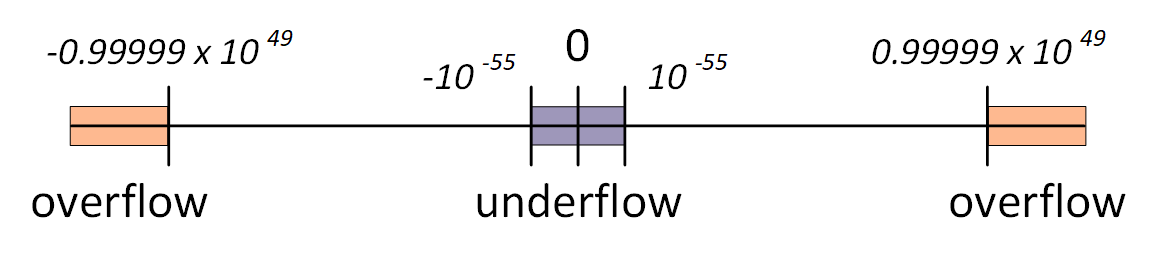
\includegraphics[scale=1]{img/flottants/floats_overflows_underflows.png}
\caption{(extrait de \og \textit{Englander: The Architecture of Computer Hardware and Systems Software} \fg{})}
}
\end{figure}
\end{center}

Ainsi, non seulement il existe une limite haute/basse sur la partie entière représentable d'un nombre, mais également sur la quantité de chiffres après la virgule.
Les nombres flottants sont donc parfois des approximations lorsqu'ils sont manipulés.
En développement, on ne teste \textit{jamais} l'égalité entre deux variables représentées par des nombres flottants, mais uniquement un écart entre elles (si cet écart est suffisamment négligeable, alors elles peuvent être considérées comme égales).

\bigskip

Lorsque l'on travaille sur les nombres à virgules, vous connaissez déjà une forme de notation dite scientifique.
On y met un unique entier entre $ 1 $ et $ 9 $ (inclus), et on l'accompagne d'une virgule suivi d'un nombre, puis on le multiplie par une puissance de $ 10 $.

\bigskip

\begin{equation*}
-2541,3945 = -2,5413945 \times 10^{3}
\label{equation:1-Notation-Scientifique}
\end{equation*}

\bigskip

Cette notation est parfois simplifiée en utilisant un $ e $ pour \textit{exposant}.

\bigskip

\begin{equation*}
0,0001337 = 1,337 \times 10^{-4} = 1,337\text{e}-4
\label{equation:2-Notation-Scientifique}
\end{equation*}

\bigskip

Ce format $ \pm \, a \times 10^{n} $ est également utilisé pour représenter les nombres dits flottants (car la virgule \og flotte \fg{} selon la puissance de 10 utilisée).
Cette notation se compose de trois éléments :

\bigskip

%\begin{center}
%\begin{tabular}{c c c c}
%\underline{$\pm$} & \underline{a} & $ \times 10 $ & \underline{$^{n}$} \\
%            signe &      mantisse &               &           exposant \\
%\end{tabular}
%\end{center}

\begin{center}
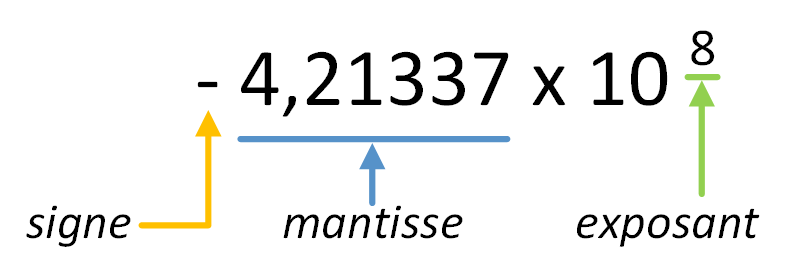
\includegraphics[scale=0.75]{img/flottants/floats_parties.png}
\end{center}

\bigskip

\begin{itemize}
\item \textit{signe} : positif ou négatif (ici \og - \fg{})
\item \textit{exposant} : la puissance de 10 (ici $ 8 $)
\item \textit{mantisse} (ou significande) : le nombre décimal (ici $ 4,21337 $)
\end{itemize}

\bigskip

Dans la notation IEEE 754, on utilise ces mêmes concepts, mais appliqués à la base 2 et avec une taille précise pour représenter chacun d'entre eux.
Ainsi, la mantisse a une valeur minimale et une valeur maximale, tout comme l'exposant.
De plus, le vocabulaire varie légèrement du fait que la norme impose quelques contraintes.
On parlera donc dans le vocabulaire formel de :

\bigskip

\begin{itemize}
\item \textit{signe} : positif ou négatif
\item \textit{exposant biaisé} : la puissance de 2, à laquelle il faut ajouter une valeur (le biais)
\item \textit{mantisse} : la partie décimale après la virgule (en ignorant le 1 de la partie entière)
\end{itemize}

\begin{figure}[ht!]
\centering{
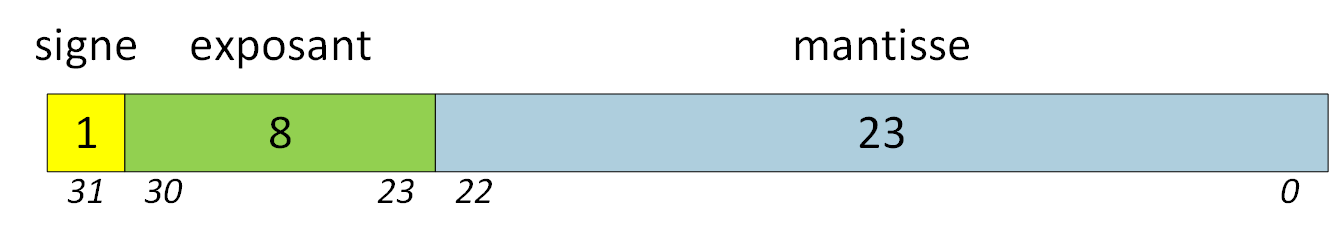
\includegraphics[scale=0.65]{img/flottants/floats_precision_single_length.png}
}
\caption{représentation des flottants IEEE 754 simple précision (32 bits)}
\end{figure}

\begin{figure}[ht!]
\centering{
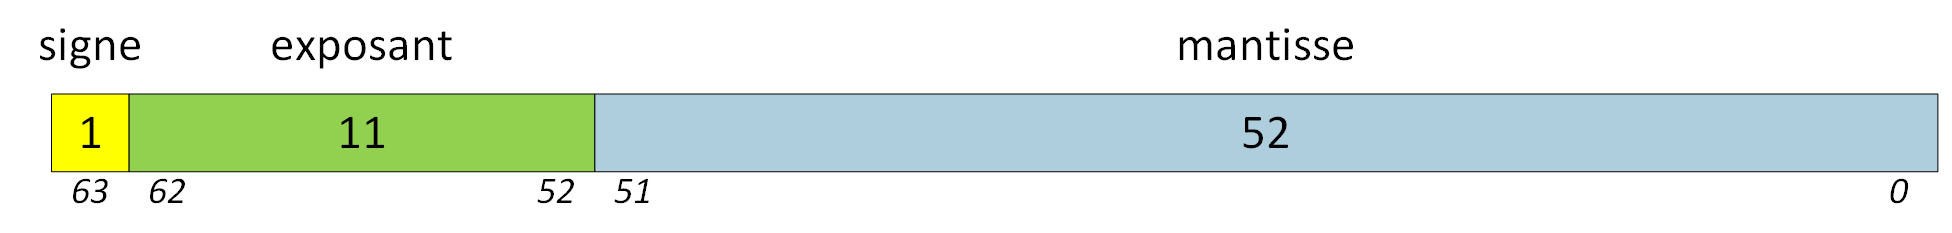
\includegraphics[scale=0.65]{img/flottants/floats_precision_double_length.png}
}
\caption{représentation des flottants IEEE 754 double précision (64 bits)}
\end{figure}


\bigskip

De plus, étant donné que les représentations numériques ont des limites, on distingue plusieurs cas dans la taille des flottants : la \textit{simple précision} (ou \textit{single precision} en anglais) sur 32 bits, la \textit{double précision} sur 64 bits, et d'autres formats que nous n'étudierons pas.
La précision fait varier la taille générale des flottants, ce qui implique que les flottants double précision couvreront plus de grandes valeurs, mais également plus de petites valeurs proches de $ 0 $, que les flottants simple précision.

\bigskip

\begin{itemize}
\item \textit{signe} : 1 bit
\item \textit{exposant} : 8 bits (simple précision), 11 bits (double précision), 15 bits (quadruple precision)
\item \textit{mantisse} : 23 bits (simple précision), 52 bits (double précision), 112 bits (quadruple precision)
\end{itemize}

\bigskip

Enfin, pour convertir les décimaux en flottants IEEE 754, il existe une convention pour les \textit{nombres normalisés} (valeur absolue supérieure à 1), et les \textit{nombre dénormalisés} (valeur absolue inférieure à 1).

\bigskip

%%%%%%%%%%%%%%%%%%%%%%%%%%%%%%%%%%%%%%

\section{Valeurs réservées}

\bigskip

La norme prévoit également une réservation de certaines valeurs clés.
Vous devez les connaître pour pouvoir les reconnaître.

\begin{center}
\begin{tabular}{ | c | c | c | c | c | }
\hline
Type & Valeur héxadécimale & Signe & Exposant & Mantisse \\
\hline
+ Zéro      & $ \$ $ 0000 0000 & 0 & $ \% 0000 \, 0000 $ & $ \% \; 000 \, 0000 \, 0000 \, 0000 \, 0000 \, 0000 $ \\
- Zéro      & $ \$ $ 8000 0000 & 1 & $ \% 0000 \, 0000 $ & $ \% \; 000 \, 0000 \, 0000 \, 0000 \, 0000 \, 0000 $ \\
\hline
+ $ \infty $  & $ \$ $ 7F80 0000 & 0 & $ \% 1111 \, 1111 $ & $ \% \; 000 \, 0000 \, 0000 \, 0000 \, 0000 \, 0000 $ \\
- $ \infty $  & $ \$ $ FF80 0000 & 1 & $ \% 1111 \, 1111 $ & $ \% \; 000 \, 0000 \, 0000 \, 0000 \, 0000 \, 0000 $ \\
\hline
NaN (borne B) & $ \$ $ \_F80 0001 & X & $ \% 1111 \, 1111 $ & $ \% \; 000 \, 0000 \, 0000 \, 0000 \, 0000 \, 0001 $ \\
NaN (borne H) & $ \$ $ \_FFF FFFF & X & $ \% 1111 \, 1111 $ & $ \% \; 111 \, 1111 \, 1111 \, 1111 \, 1111 \, 1111 $ \\
\hline
\end{tabular}
\end{center}

\bigskip


%%%%%%%%%%%%%%%%%%%%%%%%%%%%%%%%%%%%%%%%%%%%%%%%%%%%%%%%%%%%%%%%%%%%%%%%%
%%%%%%%%%%%%%%%%%%%%%%%%%%%%%%%%%%%%%%%%%%%%%%%%%%%%%%%%%%%%%%%%%%%%%%%%%
%%%%%%%%%%%%%%%%%%%%%%%%%%%%%%%%%%%%%%%%%%%%%%%%%%%%%%%%%%%%%%%%%%%%%%%%%
%%%%%%%%%%%%%%%%%%%%%%%%%%%%%%%%%%%%%%%%%%%%%%%%%%%%%%%%%%%%%%%%%%%%%%%%%

% https://www.h-schmidt.net/FloatConverter/IEEE754.html

\section{Nombres normalisés : base 10 vers IEEE 754}

\bigskip

Les nombres normalisés dans le format IEEE 754 concernent les nombres dont la valeur absolue est supérieure à $ 1 $ (mais restent inférieurs à la borne maximale gérée par la précision choisie).
L'objectif est de représenter les nombres
Voici les étapes pour convertir les nombres normalisés :

\medskip

\begin{enumerate}
\item Récupérer le signe du nombre (positif = 0, négatif = 1)
\item Séparer la partie entière de la partie décimale
\item Convertir la partie entière en binaire (sans gérer le signe)
\item Convertir la partie décimale en binaire (sans gérer le signe)
\item Fusion des parties entière et décimale en binaire tout en gardant la virgule
\item Réécriture en notation scientifique base 2
\item Calculer l'exposant pour le format IEEE 754 en l'ajoutant au biais de la précision choisie
\item Convertir l'exposant biaisé en binaire
\item Reporter la mantisse selon la précision choisie
\end{enumerate}

\bigskip

Nous traiterons ici comme exemple la valeur $ - 42,15625 $.

\bigskip

\subsection{Récupérer le signe du nombre}

\medskip

On place dans le bit de poids fort servant à coder le signe un $ 0 $ si le nombre est positif, ou un $ 1 $ si le nombre est négatif.
Dans l'ensemble des étapes suivantes, on peut ignorer le signe du nombre.

\medskip

On retient donc $ 1 $ que l'on place au bit 31 en simple précision, et au bit 63 en double précision.

Pour les étapes suivantes, on travaillera donc sur $ 42,15625 $.

\bigskip

\subsection{Séparer la partie entière de la partie décimale}

\medskip

On sépare la partie entière de la partie décimale afin de les convertir en binaire chacune de leur façon.

\medskip

$ 42,15625 $ devient donc $ 42 $ et $ 0,15625 $.

\bigskip

\subsection{Convertir la partie entière en binaire}

\medskip

On convertit la partie entière en binaire avec l'algorithme classique de division par 2.

\medskip

Dans les traitements suivants, le $ 1 $ de tête sera considéré comme implicite, donc il sera omis lors de l'écriture finale de la mantisse.
Pour le traitement suivant concernant la conversion binaire de la partie décimale, il est parfois utile de connaître le nombre de bits utilisés pour représenter cette partie (moins le $ 1 $ de tête).
Néanmoins, pour connaître le nombre de décalages nécessaires, il est nécessaire de conserver le nombre binaire tel quel.

\medskip

$ 42_{10} \; = \; 101010_{2} $

\bigskip

\subsection{Convertir la partie décimale en binaire}

\medskip

On convertit la partie décimale en binaire.
Pour cela, on effectue des multiplications successives par $ 2 $ en faisant l'extraction de la partie entière.
En effet, les bits représentent toujours des puissances de 2, mais des puissances négatives (donc $ 2^{-1} $, $ 2^{-2} $, $ 2^{-3} $, ... soit $ 0,5 $, $ 0,25 $, $ 0,125 $, ...).

\medskip

La condition d'arrêt est soit d'atteindre \og $ 1,0 $ \fg{}, soit que la taille de la partie entière convertie en binaire + le nombre de multiplication tienne sur la taille de la mantisse exploitée.
Dans notre cas, $ 42 $ est converti en $ 101010_{2} $, donc en omettant le $ 1 $ de tête, $ 01010_{2} $, celui-ci prendra 5 bits dans la mantisse.
En simple précision, la mantisse étant de 23 bits, on pourra donc placer 18 bits ($ 23 - 5 $) de nombres après la virgule.
%À la fin de la dernière multiplication applicable (la $ 18^e $), on arrondit le résultat à $ 0 $ ou $ 1 $.

S'il est impossible de représenter le nombre sur 23 bits (exemple : $ \frac{1}{3} $), on arrondit la dernière multiplication réalisable à $ 0 $ ou $ 1 $.

\medskip

\begin{center}
\begin{tabular}{c c c   m{1cm}   c }
multiplication        &         & résultat    & & entier \\
$ 0,15625 \times 2 $  &  $ = $  &  $ 0,31250 $ & & $ 0 $ \\
$ 0,3125  \times 2 $  &  $ = $  &  $ 0,6250  $ & & $ 0 $ \\
$ 0,625   \times 2 $  &  $ = $  &  $ 1,250   $ & & $ 1 $ \\
$ 0,25    \times 2 $  &  $ = $  &  $ 0,50    $ & & $ 0 $ \\
$ 0,5     \times 2 $  &  $ = $  &  $ 1,0     $ & & $ 1 $ \\
\end{tabular}
\end{center}

\medskip

On lit cette fois les multiplications dans l'ordre où elles ont été effectuées.

\medskip

$ 0,15625_{10} = 0,00101_{2} $

%\begin{tabular}{c c c   m{1cm}   c }
%multiplication       &         & résultat    & & entier
%$ 0,1337 \times 2 $  &  $ = $  &  $ 0,2674 $ & & $ 0 $
%$ 0,2674 \times 2 $  &  $ = $  &  $ 0,5348 $ & & $ 0 $
%$ 0,5348 \times 2 $  &  $ = $  &  $ 1,0696 $ & & $ 1 $
%$ 0,0696 \times 2 $  &  $ = $  &  $ 0,1392 $ & & $ 0 $
%$ 0,1392 \times 2 $  &  $ = $  &  $ 0,2784 $ & & $ 0 $
%$ 0,2784 \times 2 $  &  $ = $  &  $ 0,5568 $ & & $ 0 $
%$ 0,5568 \times 2 $  &  $ = $  &  $ 1,1136 $ & & $ 1 $
%$ 0,1136 \times 2 $  &  $ = $  &  $ 0,2272 $ & & $ 0 $
%$ 0,2272 \times 2 $  &  $ = $  &  $ 0,4544 $ & & $ 0 $
%$ 0,4544 \times 2 $  &  $ = $  &  $ 0,9088 $ & & $ 0 $
%$ 0,9088 \times 2 $  &  $ = $  &  $ 1,8176 $ & & $ 1 $
%$ 0,8176 \times 2 $  &  $ = $  &  $ 1,6352 $ & & $ 1 $
%$ 0,6352 \times 2 $  &  $ = $  &  $ 1,2704 $ & & $ 1 $
%$ 0,2704 \times 2 $  &  $ = $  &  $ 0,5408 $ & & $ 0 $
%$ 0,5408 \times 2 $  &  $ = $  &  $ 1,0816 $ & & $ 1 $
%$ 0,0816 \times 2 $  &  $ = $  &  $ 0,1632 $ & & $ 0 $
%$ 0,1632 \times 2 $  &  $ = $  &  $ 0,3264 $ & & $ 0 $
%$ 0,3264 \times 2 $  &  $ = $  &  $ 0,6528 $ & & $ 0 $ <= 1 arrondi au dessus ?
%$ 0,6528 \times 2 $  &  $ = $  &  $ 1,3056 $ & & $ 1 $
%\end{tabular}

% You entered                     : -42.1337
% Value actually stored in float  : -42.133701324462890625
% Error due to conversion         : -0.000001324462890625
% Binary Representation           : 1 10000100 01010001000100011101001
% Binary Representation           : 1 10000100 01010,001000100011101001
% Binary Representation           : 11000010001010001000100011101001
% Hexadecimal Representation      : 0xc22888e9


\bigskip

\subsection{Fusion des parties entière et décimale en binaire tout en gardant la virgule}

\medskip

On fusionne les parties entières et décimales converties en binaire, tout en conservant le placement de la virgule.

\medskip

$ 42_{10} = 101010_{2} $

\medskip

$ 0,15625_{10} = 0,00101_{2} $

\bigskip

$ 42,15625_{10} = 101010,00101_{2} $

\bigskip

\subsection{Réécriture en notation scientifique base 2}

\medskip

On déplace la virgule pour atteindre le $ 1 $ le plus à gauche de la partie entière, et on garde ce décalage comme exposant.

\medskip

$ 101010,00101_{2} = 10 \; 1010,0010 \; 1_{2} \times 2^{0} = 1,0101 \; 0001 \; 01_{2} \times 2^{5} $

\bigskip

\subsection{Calculer l'exposant en ajoutant le biais}

\medskip

On ajoute le biais (lié à la précision choisie) à l'exposant précédemment obtenu.
En simple précision, le biais est de $ 127 $. En double précision il est de $ 1023 $. En quadruple précision, il est de $ 16383 $.

\medskip

$ 1,0101000101_{2} \times 2^{5}  \; \; \Rightarrow \; \;  2^{\text{\circled{\textit{5}}}} $

\medskip

Simple précision : $ 5 + 127 = 132 $

\medskip

Double précision : $ 5 + 1023 = 1028 $

\bigskip

\subsection{Convertir l'exposant biaisé en binaire}

\medskip

On convertit en binaire l'exposant biaisé, et on le reporte dans le champ prévu.

\medskip

Simple précision (8 bits) : $ 132_{10} = \; 1000 \; 0100_{2} $

\medskip

Double précision (11 bits) : $ 1028_{10} = \; 100 \; 0000 \; 0100_{2} $

\bigskip

\subsection{Reporter la mantisse selon la précision choisie}

\medskip

On reporte la mantisse dans le champ prévu en omettant le $ 1 $ en tête : en effet, celui-ci est implicite par l'écriture scientifique en base 2.

De plus, on ajoute autant de $ 0 $ que nécessaire à droite du nombre.

\medskip

$ 1,0101000101_{2} \times 2^{5}  \; \; \Rightarrow \; \;  0101000101_{2} $

\medskip

Simple précision (23 bits) :

$ 0101 0001 0100 0000 0000 000_{2} $  \hfill  $ 010 \; 1000 \; 1010 \; 0000 \; 0000 \; 0000_{2} $  \hfill \phantom{Texte.}

\medskip

Double précision (52 bits) :

$ 0101 0001 0100 0000 0000 0000 0000 0000 0000 0000 0000 0000 0000_{2} $

$ 0101 \; 0001 \; 0100 \; 0000 \; 0000 \; 0000 \; 0000 \; 0000 \; 0000 \; 0000 \; 0000 \; 0000 \; 0000_{2} $

\bigskip

\subsection{Résultat}

\bigskip

Enfin, on peut fusionner l'ensemble des trois champs pour représenter un nombre normalisé au format IEEE 754 : signe ($ 1 $), exposant ($ 1000 0100_{2} $ ou $ 100 0000 0100_{2} $), mantisse

\medskip


Simple précision (32 bits) :

$ 1 1000 0100 0101 0001 0100 0000 0000 000_{2} $  \hfill  $ 1\underline{100 \; 0010 \; 0}010 \; 1000 \; 1010 \; 0000 \; 0000 \; 0000_{2} $

\medskip

Double précision (64 bits) :

$ 1 100 0000 0100 0101 0001 0100 0000 0000 0000 0000 0000 0000 0000 0000 0000 0000_{2} $

$ 1\underline{100 \; 0000 \; 0100} \; 0101 \; 0001 \; 0100 \; 0000 \; 0000 \; 0000 \; 0000 \; 0000 \; 0000 \; 0000 \; 0000 \; 0000 \; 0000_{2} $


\bigskip


Simple précision (32 bits) : $ -42.15625_{10} = \text{C}228\text{A}000_{16} $  \hfill $ \text{C}228 \; \text{A}000_{16} $  \hfill \phantom{Texte.}

\medskip

Double précision (64 bits) : $ -42.15625_{10} = \text{C}045140000000000_{16} $  \hfill  $ \text{C}045 \; 1400 \; 0000 \; 0000_{16}$  \hfill \phantom{Texte}


% You entered                     : -42.15625
% Value actually stored in float  : -42.15625
% Error due to conversion         : 0.00000
% Binary Representation           : 1 10000100 01010001010000000000000
% Binary Representation           : 11000010001010001010000000000000
% Hexadecimal Representation      : 0xc228a000

\bigskip

%%%%%%%%%%%%%%%%%%%%%%%%%%%%%%%%%%%%%%%%%%%%%%%%%%%%%%%%%%%%%%%%%%%%%%%%%
%%%%%%%%%%%%%%%%%%%%%%%%%%%%%%%%%%%%%%%%%%%%%%%%%%%%%%%%%%%%%%%%%%%%%%%%%
%%%%%%%%%%%%%%%%%%%%%%%%%%%%%%%%%%%%%%%%%%%%%%%%%%%%%%%%%%%%%%%%%%%%%%%%%
%%%%%%%%%%%%%%%%%%%%%%%%%%%%%%%%%%%%%%%%%%%%%%%%%%%%%%%%%%%%%%%%%%%%%%%%%


\section{Nombres normalisés : IEEE 754 vers base 10}

\bigskip

Pour interpréter une valeur flottante IEEE 754, il est nécessaire de s'assurer tout d'abord qu'il ne s'agisse pas d'une des valeurs réservées, particulièrement les NaN (\textit{Not a Number} en anglais) indiquant que la valeur n'est pas un nombre, et les valeurs infinies.
Pour cela, il faut effectuer les mêmes étapes en sens inverse que pour la conversion, et s'intéresser à la valeur de l'exposant en priorité : un exposant à la valeur maximale (c'est-à-dire qu'en binaire il n'y aura que des $ 1 $) indiquera une valeur réservée (pour rappel : l'infini ou NaN).
Un exposant et une mantisse à $ 0 $ indiqueront qu'il s'agit de la valeur zéro.

\medskip

Voici les étapes pour convertir les nombres normalisés :

\begin{enumerate}
\item Séparer les champs
\item Retrouver le signe
\item Convertir l'exposant biaisé en base 10
\item Convertir la mantisse en base 10
\item Calculer la valeur décimale
\end{enumerate}

\bigskip

\subsection{Séparer les champs}

\medskip

La première étape consiste simplement à séparer les champs selon la précision du flottant étudié.

\bigskip

\begin{tabular}{| l | c | c | c |}
\hline
         & simple précision (32 bits) & double précision (64 bits) & quadruple précision (128 bits) \\
\hline
signe    & 1 bit   & 1 bit   & 1 bit \\
\hline
exposant & 8 bits  & 11 bits & 15 bits \\
\hline
mantisse & 23 bits & 52 bits & 112 bits \\
\hline
\end{tabular}

\bigskip
\bigskip

$ \text{BA}13 \; \text{C}700_{16} $ = $ 1\underline{011 \; 1010 \; 0}001 \; 0011 \; 1100 \; 0111 \; 0000 \; 0000_{2} $  \hfill simple précision (32 bits) \hfill \phantom{Texte.}

\bigskip
\bigskip

\begin{tabular}{l c l}
Signe (1 bit) :      & $ 1_{2} $            & \\
Exposant (8 bits) :  & $ 0111 \; 0100_{2} $ & Exposant classique (ni nul ni au max)\\
Mantisse (23 bits) : & $ 001 \; 0011 \; 1100 \; 0111 \; 0000 \; 0000_{2} $ & \\
\end{tabular}

\bigskip
\bigskip

Au delà des valeurs réservées, la formule générale à appliquer est la suivante :
\begin{center}
$ (-1)^{\text{signe}} \times (1 + \text{mantisse}) \times 2^{\text{exposant - biais}} $
\end{center}


\bigskip

\subsection{Retrouver le signe}

\medskip

On observe simplement si le bit de signe est à $ 1 $ (nombre négatif) ou à $ 0 $ (nombre positif).

\medskip

Signe : $ 1 \; \; \; \; $ (nombre négatif)

\bigskip

\subsection{Convertir l'exposant biaisé en base 10}

\medskip

On convertit l'exposant biaisé binaire en décimal afin de pouvoir soustraire le biais.

$ 0111 \; 0100_{2} = 116_{10} $

\bigskip

\subsection{Convertir la mantisse en base 10}

\medskip

La mantisse est précédée d'un \og $ 0, $ \fg{} afin de retrouver les puissances de $ 2 $ associées.

\medskip

$ 001 \; 0011 \; 1100 \; 0111 \; 0000 \; 0000_{2}  \; \; \Rightarrow \; \; 0,0010 \; 0111 \; 1000 \; 111_{2} $

\medskip

%$ 0,0010 \; 0111 \; 0110 \; 111_{2} = 2^{-3} + 2^{-6} + 2^{-7} + 2^{-8} + 2^{-10} + 2^{-11} + 2^{-13} + 2^{-14} + 2^{-15} $
\begin{tabular}{l l l}
$ 0,0010 \; 0111 \; 1000 \; 111_{2} $ & $ = $ & $ 0 \times 2^{-1} \; + \; 0 \times 2^{-2} \; + \; 1 \times 2^{-3} \; + \; 0 \times 2^{-4} \; + \; ... \; + \; 1 \times 2^{-15} $ \\
 & & \\
                                      & $ = $ & $ 2^{-3} + 2^{-6} + 2^{-7} + 2^{-8} + 2^{-9} + 2^{-13} + 2^{-14} + 2^{-15} $ \\
 & & \\
                                      & $ = $ & $ 0,125 \, + \, 0,015625 \, + \, 0,0078125 \, + \, 0,00390625 \, + \, 0,001953125 $ \\
                                      &       & $ + \; 0,0001220703125 \, + \, 0,00006103515625 \, + \, 0,000030517578125 $ \\
 & & \\
                                      & $ = $ & $ 0,154510498046875 $
\end{tabular}

\bigskip

\subsection{Calculer la valeur décimale}

\medskip

On applique enfin la formule suivante avec les valeurs trouvées et le biais associé à la précision :

\begin{table}[ht!]
  \centering
  \begin{minipage}{0.45\textwidth}
    \centering

\begin{center}
$ (-1)^{\text{signe}} \times (1 + \text{mantisse}) \times 2^{\text{exposant - biais}} $
\end{center}

  \end{minipage}
  \hfillx
  \begin{minipage}{0.45\textwidth}
    \centering

\begin{tabular}{| l | c |}
\hline
Précision & Biais \\
\hline
Simple (32 bits)  & 127 \\
\hline
Double (64 bits)  & 1023 \\
\hline
Quadruple (128 bits) & 16383 \\
\hline
\end{tabular}

  \end{minipage}
\end{table}


\begin{center}
$ (-1)^{1} \times (1 + 0,154510498046875) \times 2^{116 - 127} $

\smallskip
$ = $
\smallskip

$ (-1) \times (1,154510498046875) \times 2^{-11} $

\smallskip
$ = $
\smallskip

$ -1,154510498046875 \times 2^{-11} $

\smallskip
$ = $
\smallskip

$ -0,00056372582912445068 $

\smallskip
$ = $
\smallskip

\textit{(notation scientifique)} $ -5,6372582912445068 \times 10^{-4} $
\end{center}

Il ne faut surtout pas oublier qu'il s'agit d'une approximation : la valeur initiale qui était manipulée par l'ordinateur a été transformée en format IEEE 754 qui a provoqué une limitation dans la quantité de chiffres après la virgule.
Les opérations elles-mêmes de conversion peuvent également souffrir d'un manque de précision.

\medskip

En conclusion, le nombre retrouvé en fin de conversion n'est pas nécessairement la valeur exacte initialement manipulée.

\medskip

Si un programme implique de manipuler et modifier plusieurs fois de suite un nombre flottant, il vaut mieux trouver une autre représentation, et ne convertir en flottant que la valeur finale (par exemple en créant un type abstrait \og \textit{fraction} \fg{} qui sera utilisé dans le programme, et uniquement lorsque les traitements auront été terminés, la valeur sera convertie en flottant).

%\medskip

%Un autre facteur d'imprécision provient également de l'ordre pour effectuer chacune de ces étapes : si l'application de l'exposant se fait trop tôt, dans notre cas où l'exposant est négatif ($ -11 $), alors les valeurs seront beaucoup plus petites et nécessiteront des registres plus longs.

\bigskip

%%%%%%%%%%%%%%%%%%%%%%%%%%%%%%%%%%%%%%%%%%%%%%%%%%%%%%%%%%%%%%%%%%%%%%%%%
%%%%%%%%%%%%%%%%%%%%%%%%%%%%%%%%%%%%%%%%%%%%%%%%%%%%%%%%%%%%%%%%%%%%%%%%%
%%%%%%%%%%%%%%%%%%%%%%%%%%%%%%%%%%%%%%%%%%%%%%%%%%%%%%%%%%%%%%%%%%%%%%%%%
%%%%%%%%%%%%%%%%%%%%%%%%%%%%%%%%%%%%%%%%%%%%%%%%%%%%%%%%%%%%%%%%%%%%%%%%%

\clearpage

%%%%%%%%%%%%%%%%%%%%%%%%%%%%%%%%%%%%%%%%%%%%%%%%%%%%%%%%%%%%%%%%%%%%%%%%%
%%%%%%%%%%%%%%%%%%%%%%%%%%%%%%%%%%%%%%%%%%%%%%%%%%%%%%%%%%%%%%%%%%%%%%%%%
%%%%%%%%%%%%%%%%%%%%%%%%%%%%%%%%%%%%%%%%%%%%%%%%%%%%%%%%%%%%%%%%%%%%%%%%%
%%%%%%%%%%%%%%%%%%%%%%%%%%%%%%%%%%%%%%%%%%%%%%%%%%%%%%%%%%%%%%%%%%%%%%%%%

\section{Nombres dénormalisés}

\bigskip

Les nombres dénormalisés (\textit{subnormal numbers}, \textit{denormalized numbers}, ou \textit{denormals} en anglais) concernent les nombres dont la valeur absolue est inférieure strictement à $ 1 $ (c'est-à-dire les nombres tels que : $ -1 < n < 1 $).
Plus précisément, ils servent à représenter des valeurs proches de $ 0 $, aux extrêmités de la représentation normalisée.
%Comme ces nombres ont un $ 0 $ comme chiffre entier, on ne peut pas les représenter avec une mantisse dont un  $ 1 $ est implicite (celui qui est ajouté/retiré lors de la conversion).

\medskip

Dans le format binaire, on reconnait un nombre comme dénormalisé si son exposant est nul (il ne contient que des $ 0 $) et sa mantisse est non nulle.
En effet, si la mantisse et l'exposant sont nuls, alors cela représente la valeur réservée $ 0 $.

\medskip

\begin{center}
\begin{tabular}{ | c | c | c | c | c | }
\hline
Type & Valeur héxadécimale & Signe & Exposant & Mantisse \\
\hline
$\pm$ Zéro       & $ \$ $ {\_000 0000} & X & $ \% 0000 \, 0000 $ & $ \% \; 000 \, 0000 \, 0000 \, 0000 \, 0000 \, 0000 $ \\
\hline
Dénormalisé (B)  & $ \$ $ {\_000 0001} & X & $ \% 0000 \, 0000 $ & $ \% \; 000 \, 0000 \, 0000 \, 0000 \, 0000 \, 0001 $ \\
Dénormalisé (H)  & $ \$ $ {\_07F FFFF} & X & $ \% 0000 \, 0000 $ & $ \% \; 111 \, 1111 \, 1111 \, 1111 \, 1111 \, 1111 $ \\
\hline
Normalisé (B)    & $ \$ $ {\_080 0000} & X & $ \% 0000 \, 0001 $ & $ \% \; 000 \, 0000 \, 0000 \, 0000 \, 0000 \, 0000 $ \\
Normalisé (H)    & $ \$ $ {\_F7F FFFF} & X & $ \% 1111 \, 1110 $ & $ \% \; 111 \, 1111 \, 1111 \, 1111 \, 1111 \, 1111 $ \\
\hline
$\pm \, \infty $ & $ \$ $ {\_F80 0000} & X & $ \% 1111 \, 1111 $ & $ \% \; 000 \, 0000 \, 0000 \, 0000 \, 0000 \, 0000 $ \\
\hline
NaN (borne B)    & $ \$ $ {\_F80 0001} & X & $ \% 1111 \, 1111 $ & $ \% \; 000 \, 0000 \, 0000 \, 0000 \, 0000 \, 0001 $ \\
NaN (borne H)    & $ \$ $ {\_FFF FFFF} & X & $ \% 1111 \, 1111 $ & $ \% \; 111 \, 1111 \, 1111 \, 1111 \, 1111 \, 1111 $ \\
\hline
\end{tabular}
\end{center}

\medskip

Ces nombres impliquent deux changements majeurs dans leur conversion :
\begin{itemize}
\item la mantisse ne contient pas de $ 1 $ implicite (celui ajouté/retiré avant la virgule lors de la conversion de la mantisse)
\item on ajoute $ 1 $ à la soustraction entre l'exposant (toujours à $ 0 $) et le biais
\end{itemize}
%Ainsi, le format de sortie en binaire change.

\bigskip

%Nous ne verrons pas en détails comment obtenir ces nombres, mais vous devrez savoir les repérer.

Pour rappel, les nombres normalisés sont représentés par cette formule :
\begin{center}
$ (-1)^{\text{signe}} \times (1 + \text{mantisse}) \times 2^{\text{exposant - biais}} $
\end{center}

\medskip

Mais pour les dénormalisés, on utilise cette formule :
\begin{center}
$ (-1)^{\text{signe}} \times (0 + \text{mantisse}) \times 2^{\text{exposant - biais + 1}} $

\smallskip
$ = $
\smallskip

$ (-1)^{\text{signe}} \times \text{mantisse} \times 2^{\text{1 - biais}} $
\end{center}

Si on gardait le format normalisé, en multipliant par \og \textit{1,mantisse} \fg{} on obtiendrait uniquement des valeurs proches de $ 2^{1 - biais} $.
Alors qu'en appliquant l'usage du \og \textit{0,mantisse} \fg{} on se rend compte que le résultat de la multiplication par $ 2^{1 - biais} $ peut offrir des valeurs beaucoup plus petites que seule la mantisse contrôle.

\medskip

Vous pouvez déduire de ces explications que la représentation de $ 0 $ est en réalité associée aux dénormalisés, car si on utilisait la représentation normalisée, alors la mantisse à $ 0 $ contiendrait tout de même le $ 1 $ implicite (ce qui ne ferait pas une valeur nulle).



%\bigskip
\clearpage


\subsection{Bornes dénormalisées}

\medskip

Essayons de trouver le plus petit nombre positif non-nul dénormalisé et le plus grand.

\bigskip

\subsubsection{Borne inférieure}

Le plus petit nombre positif non-nul dénormalisé en simple précision (32 bits) est :

\medskip

$ 0000 \; 0001_{16} $ = $ 0\underline{000 \; 0000 \; 0}000 \; 0000 \; 0000 \; 0000 \; 0000 \; 0001_{2} $

\bigskip

\begin{tabular}{l c l}
Signe (1 bit) :      & $ 0_{2} $            & \\
Exposant (8 bits) :  & $ 0000 \; 0000_{2} $ & Exposant nul (dénormalisé)\\
Mantisse (23 bits) : & $ 000 \; 0000 \; 0000 \; 0000 \; 0000 \; 0001_{2} $ & \\
\end{tabular}

\bigskip

\begin{center}
$ (-1)^{\text{signe}} \times \text{mantisse} \times 2^{\text{1 - biais}} $

\smallskip
$ = $
\smallskip

$ (-1)^{\text{0}} \times 2^{-23} \times 2^{1 - 127} $

\smallskip
$ = $
\smallskip

$ 2^{-23} \times 2^{-126} $

\smallskip
$ = $
\smallskip

$ 2^{-149} $
\end{center}

Le plus petit nombre positif non-nul dénormalisé en simple précision est donc $ 2^{-149} $ (soit environ $ 1,4 \times 10^{-45} $)


\bigskip


\subsubsection{Borne supérieure}

Le plus grand nombre positif non-nul dénormalisé en simple précision (32 bits) est :

\medskip

$ 007\text{F} \; \text{FFFF}_{16} $ = $ 0\underline{000 \; 0000 \; 0}111 \; 1111 \; 1111 \; 1111 \; 1111 \; 1111_{2} $

\bigskip

\begin{tabular}{l c l}
Signe (1 bit) :      & $ 0_{2} $            & \\
Exposant (8 bits) :  & $ 0000 \; 0000_{2} $ & Exposant nul (dénormalisé)\\
Mantisse (23 bits) : & $ 111 \; 1111 \; 1111 \; 1111 \; 1111 \; 1111_{2} $ & \\
\end{tabular}

\bigskip

\begin{center}
$ (-1)^{\text{signe}} \times \text{mantisse} \times 2^{\text{1 - biais}} $

\smallskip
$ = $
%\smallskip
%
\[ (-1)^{\text{0}} \times ( \sum_{n=1}^{23} 2^{-n} ) \times 2^{1 - 127} \]
%
\smallskip
$ = $
\smallskip

$ (2^{-1} + ... + 2^{-23} ) \times 2^{-126} $

\smallskip
$ \approx $
\smallskip

$ 0,999999988 \times 2^{-126} $
\end{center}

Le plus grand nombre positif non-nul dénormalisé en simple précision est proche de $ 0,999999988 \times 2^{-126} $ (soit environ $ 1,175 494 21 \times 10^{-45} $), ce qui se rapproche du plus petit nombre normalisé ($ 1,0 \times 2^{-126} $).


\bigskip

\vfillFirst

\vfillLast

\begin{center}
\textit{Ce document et ses illustrations ont été réalisés par Fabrice BOISSIER en novembre 2022}

\textit{(dernière mise à jour septembre 2023)}
\end{center}

\end{document}


% Lawrence Stewart
% Former Research Staff at Xerox PARC (1977–1984)Author has 9.1K answers and 14.8M answer views2y
%
% Topic: How do I add IEEE 754 floating point numbers?
%
% Way back around 1980, I wrote the microcode to make IEEE floating point work on the Xerox Alto, so I know something about this.
%
% Adding floating point is somewhat twisty.
%
% 1) unpack the numbers into separate sign exponent and mantissa values. Some versions will use two’s complement for the mantissa, to avoid separate sign bits.
% 2) figure out which exponent is smaller, and shift the corresponding mantissa to the right by the difference between the exponents.
% 3) add the (now aligned) mantissas
% 4) normalize the number, by shifting the sum left or right to align the leading bit. Change the exponent of the result by the number of normalization shifts. Special handling here for exponent underflow!
% 5) round the result according to the rounding mode
% 6) renormalize the number, in case the rounding changed it
% 7) repack the separate sign, exponent, and mantissa into the correct IEEE format.
% 8) Don’t forget to deal with NaN, Infinity, trapping, gradual underflow, etc.
%
% Good luck with this. Working on a floating point math emulation package will teach you quite a lot about arithmetic.
%
% PS I had a complete software version, and microcode to handle the common cases of add, subtract, and multiply. I actually implemented gradual underflow, which happens surprisingly often. I didn’t have space in the microcode so this case trapped to software, which was very slow. Ed Fiala added “underflow to zero” mode, which makes these cases run fast, but offends the purists.
